\documentclass{article}
\usepackage{graphicx} % Load the graphicx package

\begin{document}

\title{Exercício 7} 
\author{Arthur Felipe Reis Souza}
\date{\today}
\maketitle

\section{Introduction}

As redes neurais do tipo RBF (Radial Basis Function) são redes neurais com uma camada de entrada, uma camada intermediária e uma camada de saída. A camada intermediária desse tipo de rede aplica N (N é o número de neurônios da camada intermediária) funções radiais sobre os dados de entrada, gerando uma saída H que alimentará a camada de saída. Uma função radial é uma função que mensura a distância entre os pontos e um valor arbitrário. A distância pode ser entendida como uma medida de dissimilaridade entre dois ou mais valores. Há várias métricas de distâncias que podem ser utilizadas, sendo elas: Euclidean distance, Manhattan distance, Minowski distance (forma generalizada das duas anteriores). Portanto, a ideia principal das redes do tipo RBF é: pegar as entradas da rede e aplicar sobre essa entrada um conjunto de N funções radiais (função gaussiana é comumente utilizada). A saída de cada função radial será combinada linearmente com os parâmetros da camada de saída da rede, que poderá aplicar uma função de ativação sigmoidal ou identidade sobre essa combinação.

\vspace{20pt}

\begin{center}

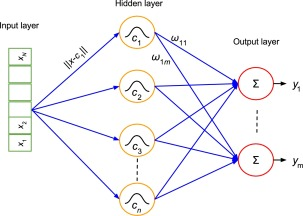
\includegraphics[height=2in]{/home/arthur/Desktop/RNA_BRAGA/RBF/RBF.jpg}

\end{center}

Faz-se mister, portanto, encontrar a localização dos centros, ou do valor central dessas funções radiais que irão aplicar, sobre os dados de entrada, uma função de dissimilaridade. Para encontrar os pontos centrais dessas funções radiais, foi utilizado um método de clustering (agrupamento) de dados chamado KMeans. O algoritmo de clustering KMeans é um algoritmo de aprendizado não supervisionado (sem informações diretas da saída), e tem por objetivo agrupar os dados em K clusters. A lógica do algoritmo KMeans é: definir as coordenadas iniciais dos K clusters e calcular a distância de cada ponto à esses clusters. Cada ponto será atribuído ao cluster mais próximo, e fazendo isso para todos os pontos teremos K agrupamentos. Após ter todos os pontos agrupados, os centros de cada cluster irão se mover para o ponto médio entre os pontos de cada agrupamento. Esse método é iterativo e não supervisionado, ou seja, irá parar de reagrupar os dados apenas perante a um critério de parada que será obtido com a minimização da discrepância entre as variâncias de cada cluster.

\vspace{20pt}

A primeira parte do exercícios 7 consiste em utilizar, nos dados obtidos no último Exercício ELM, o algoritmo KMeans para agrupar os mesmos. Após aplicar o algoritmo KMeans, usando K = 5, obtemos os seguintes resultados abaixo : 

\vspace{10pt}




\subsection{2dnormals}

\vspace{10pt}

Dados para K = 5, dataset normals : 

\vspace{10pt}

\begin{center}

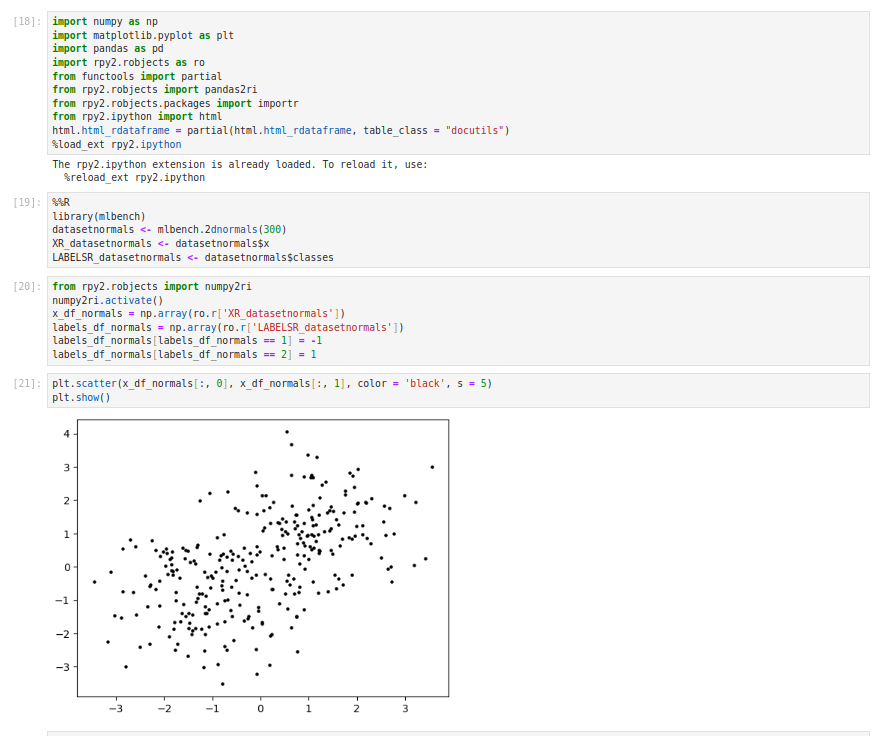
\includegraphics[height=2in]{normals_gen.png}
    
\end{center}

\vspace{10pt}

\begin{center}

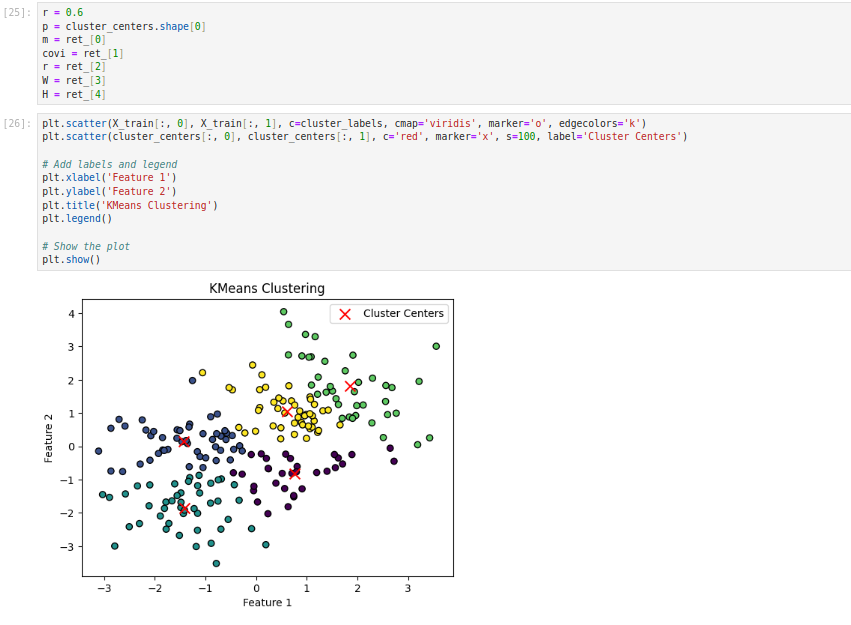
\includegraphics[height=2in]{normals_cluster.png}
        
\end{center}

\vspace{10pt}

A superfície de separação para K = 5 está registrada abaixo : 

\vspace{10pt}

\begin{center}

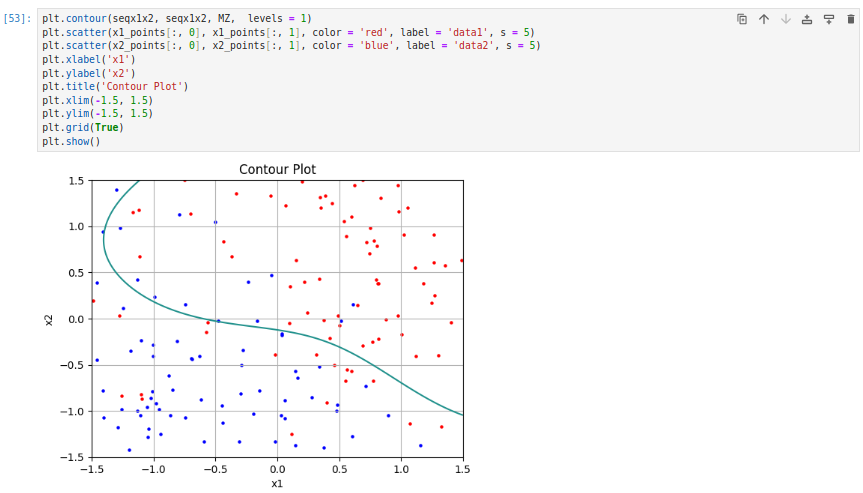
\includegraphics[height=2in]{/home/arthur/Desktop/RNA_BRAGA/ex07/normals_k5.png}
            
\end{center}

\vspace{10pt}

Aumentando muito o valor de K teoricamente levaria o modelo ao overfitting. Porém, esse conjunto de dados é facilmente separável, e não foi possível observar um overfitting visualmente, porém com um K muito grande o modelo erra mais nos dados de teste. O valor de K que levará o modelo a ter uma melhor performance é obtido com o algoritmo de Grid Search Cross-Validation, e está registrado abaixo : 

\vspace{10pt}

\begin{center}

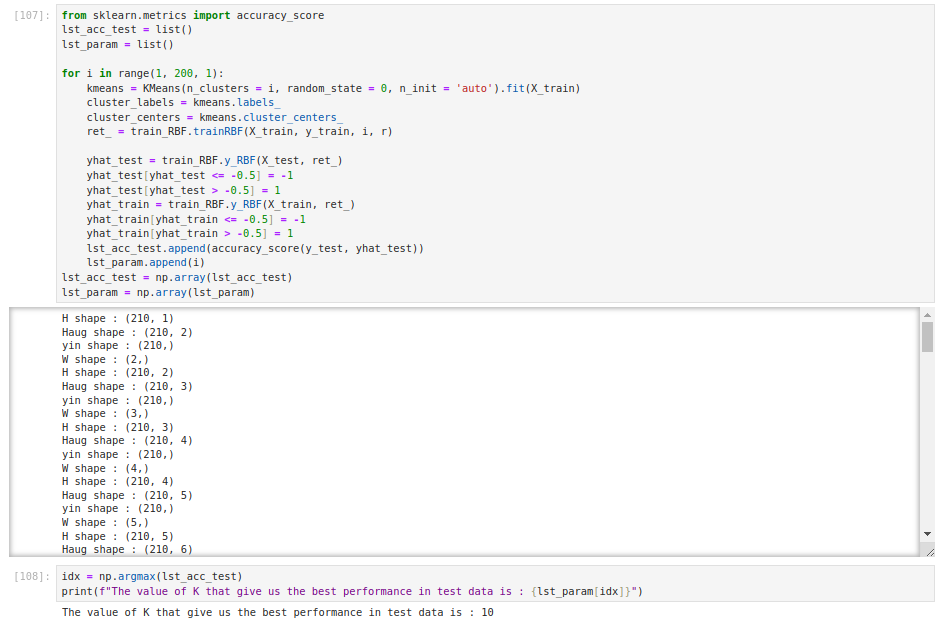
\includegraphics[height=2in]{/home/arthur/Desktop/RNA_BRAGA/ex07/bestK_normals.png}
            
\end{center}



\vspace{20pt}



\subsection{xor}

\vspace{10pt}

Dados para K = 5, dataset xor : 

\vspace{10pt}

\begin{center}

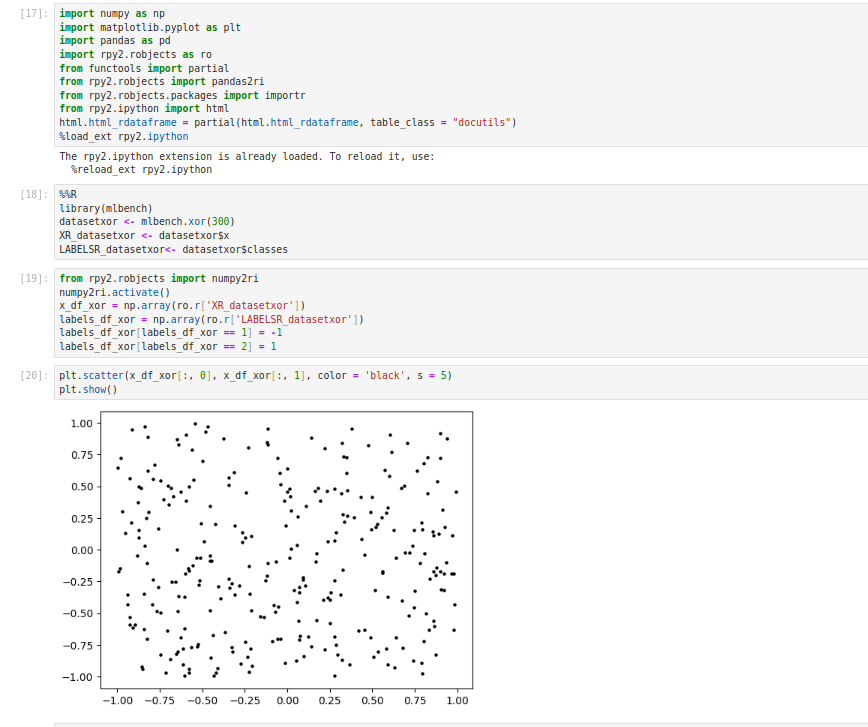
\includegraphics[height=2in]{xor_data.png}
    
\end{center}

\vspace{10pt}

\begin{center}

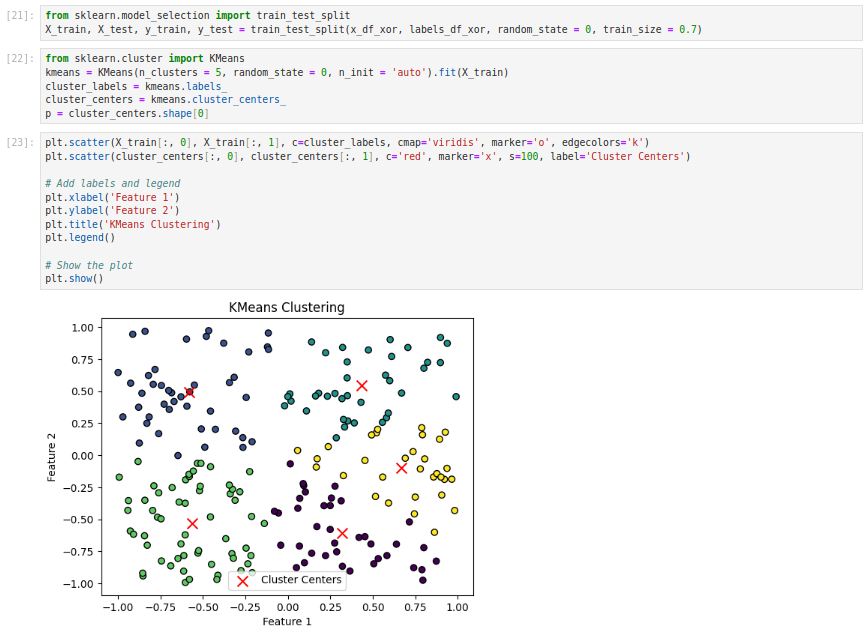
\includegraphics[height=2in]{xor_cluster.png}
        
\end{center}

\vspace{10pt}

A superfície de separação para K = 5 está registrada abaixo : 

\vspace{10pt}

\begin{center}

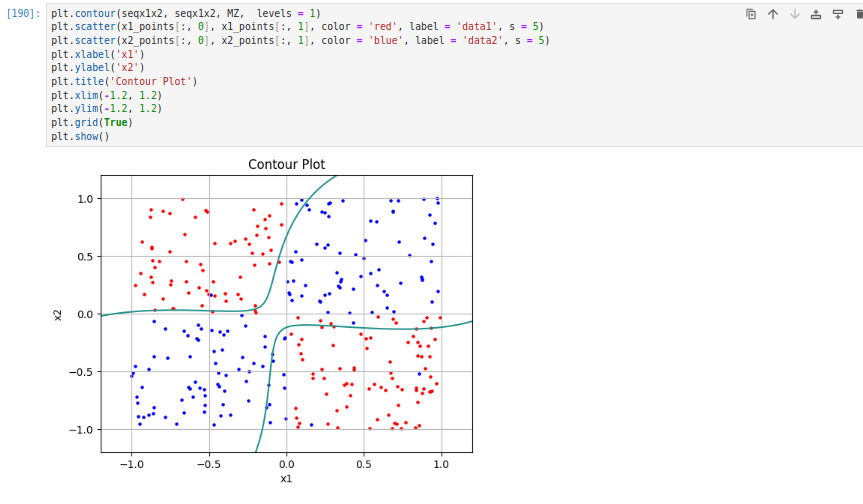
\includegraphics[height=2in]{/home/arthur/Desktop/RNA_BRAGA/ex07/xor_k5.png}
            
\end{center}

\vspace{10pt}

Aumentando muito o valor de K teoricamente levaria o modelo ao overfitting. O valor ideal de K é obtido com o metodo Grid Search CV e está registrado abaixo : 

\vspace{10pt}

\begin{center}

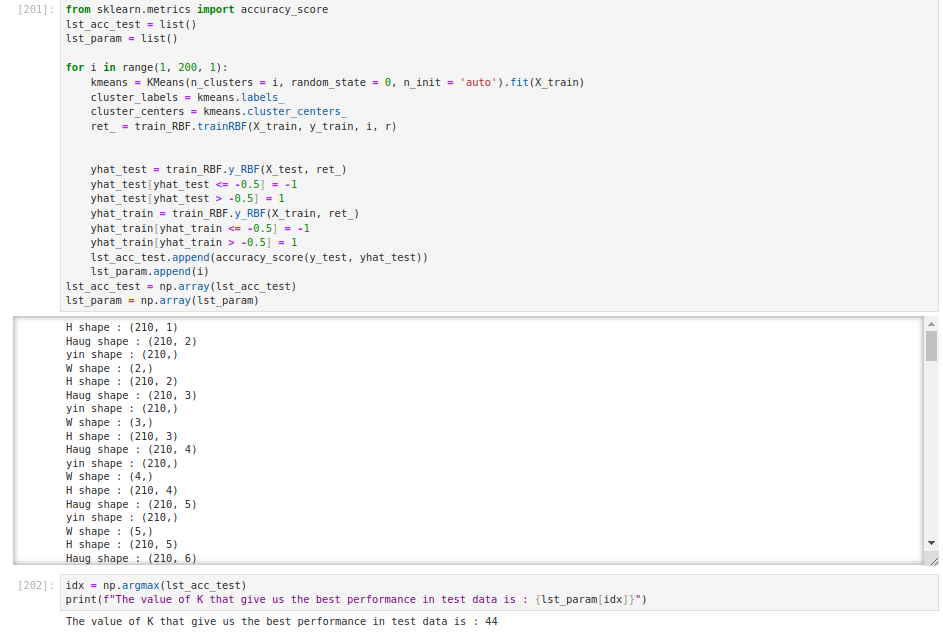
\includegraphics[height=2in]{/home/arthur/Desktop/RNA_BRAGA/ex07/best_k_xor.png}
                
\end{center}



\vspace{20pt}



\subsection{circle}

\vspace{10pt}

Dados para K = 5, dataset circle : 

\vspace{10pt}

\begin{center}

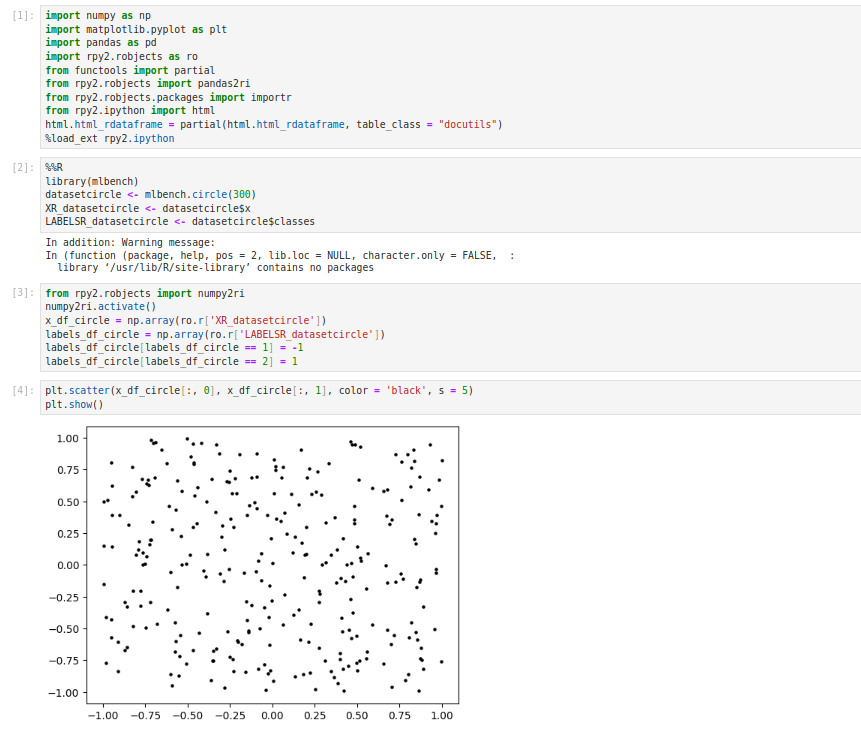
\includegraphics[height=2in]{circle_data.png}
    
\end{center}

\vspace{10pt}

\begin{center}

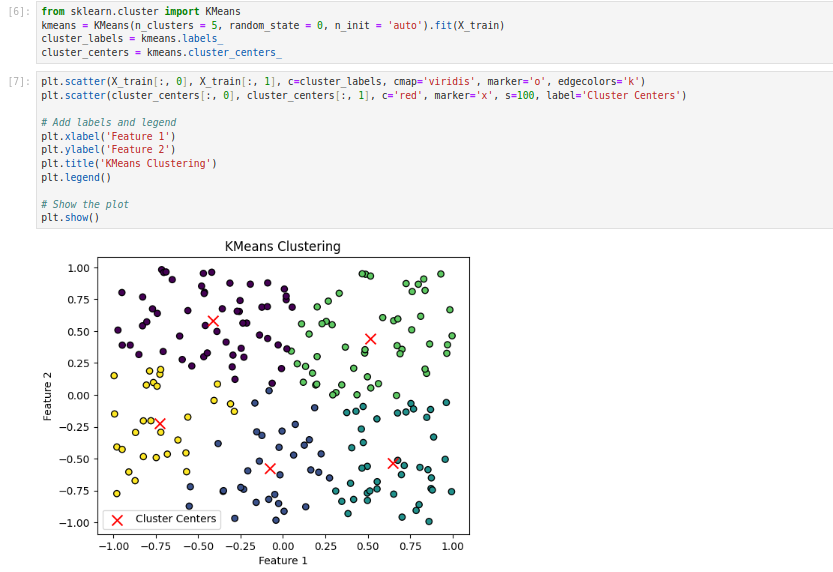
\includegraphics[height=2in]{circle_cluster.png}
        
\end{center}

\vspace{10pt}

A superfície de separação para K = 5 está registrada abaixo : 

\vspace{10pt}

\begin{center}

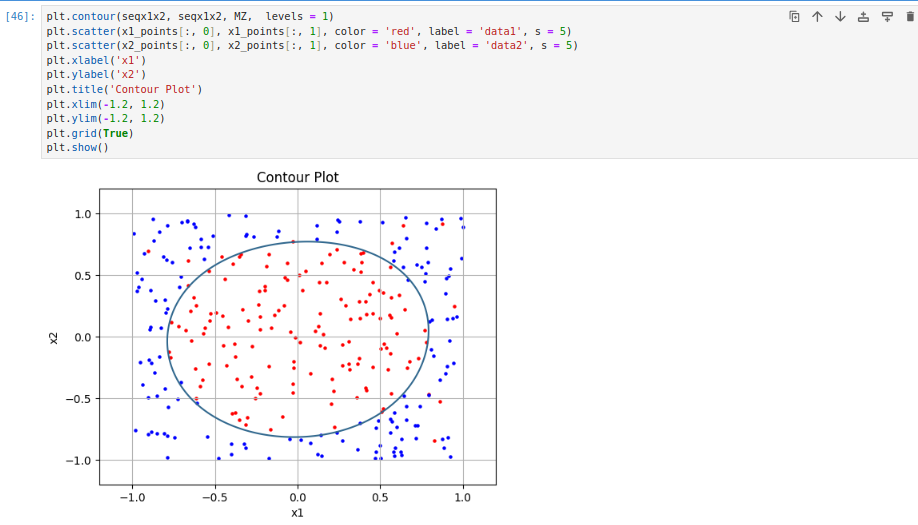
\includegraphics[height=2in]{/home/arthur/Desktop/RNA_BRAGA/ex07/circle_k5.png}
            
\end{center}

\vspace{10pt}

Aumentando muito o valor de K teoricamente levaria o modelo ao overfitting. O valor ideal de K é obtido com o metodo Grid Search CV e está registrado abaixo : 

\vspace{10pt}

\begin{center}

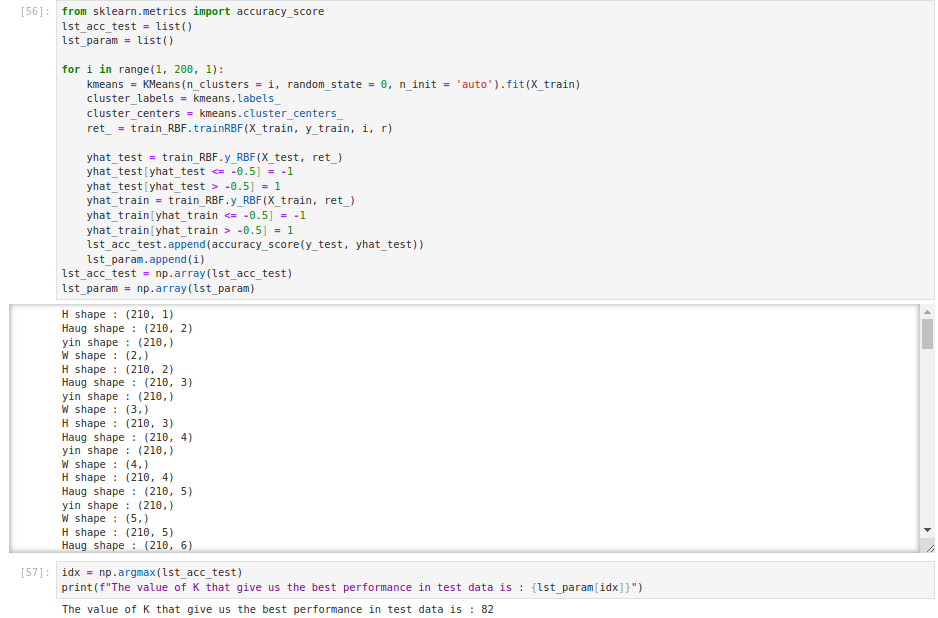
\includegraphics[height=2in]{/home/arthur/Desktop/RNA_BRAGA/ex07/best_k_circle.png}
                
\end{center}



\vspace{20pt}



\subsection{spirals}

\vspace{10pt}

Dados para K = 5, dataset spirals : 

\vspace{10pt}

\begin{center}

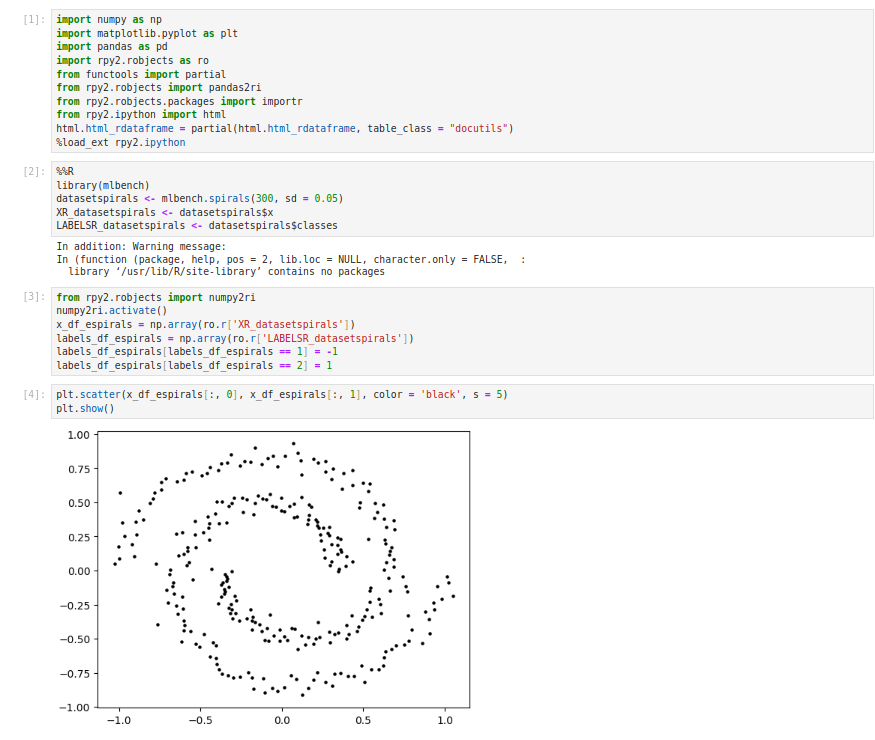
\includegraphics[height=2in]{spirals_data.png}
    
\end{center}

\vspace{10pt}

\begin{center}

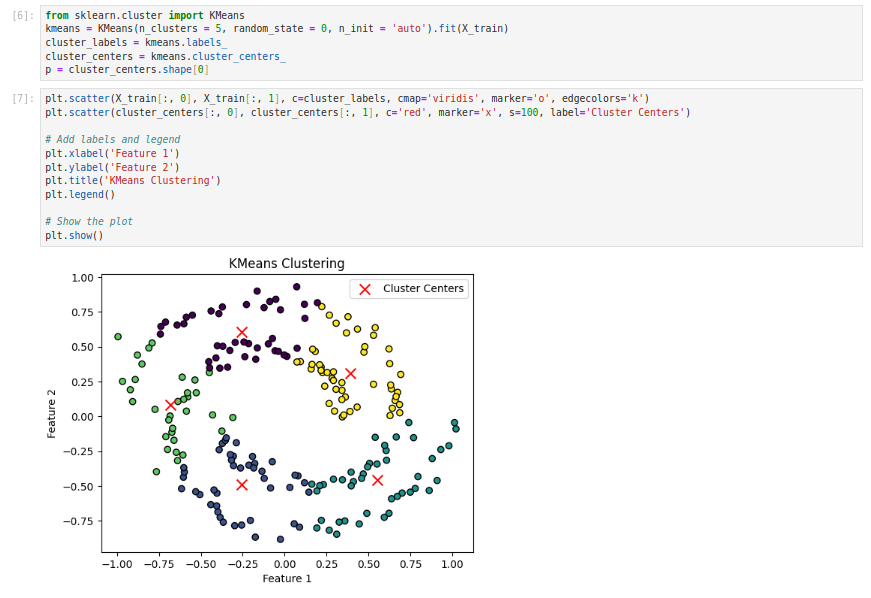
\includegraphics[height=2in]{spirals_cluster.png}
        
\end{center}

\vspace{10pt}

A superfície de separação para K = 5 está registrada abaixo : 

\vspace{10pt}

\begin{center}

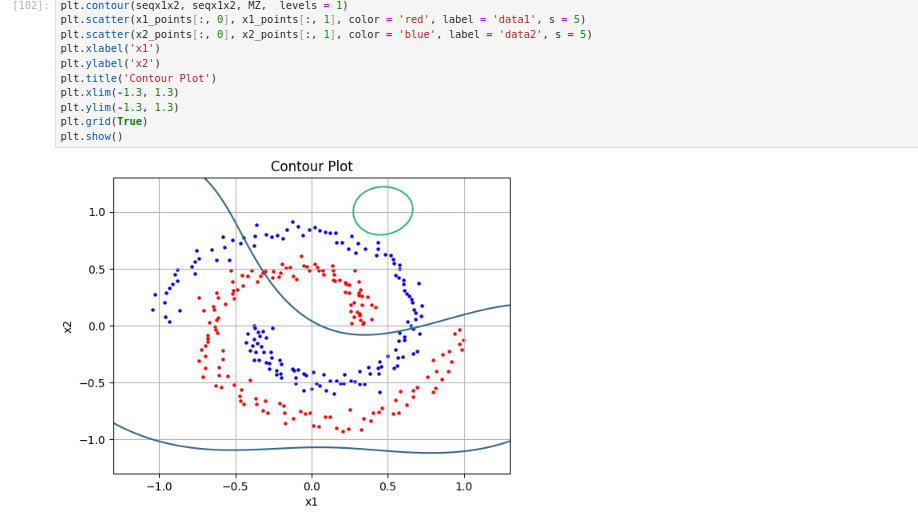
\includegraphics[height=2in]{/home/arthur/Desktop/RNA_BRAGA/ex07/spirals_k5.png}
            
\end{center}

\vspace{10pt}

Aumentando muito o valor de K teoricamente levaria o modelo ao overfitting. Como pode ser observado para K = 5, o modelo não faz uma boa aproximação. Para encontrar o melhor valor de K foi utilizado o algoritmo de Grid, que registra abaixo o melhor valor de K e também a superfície de separação para esse valor de K.

\vspace{10pt}

\begin{center}

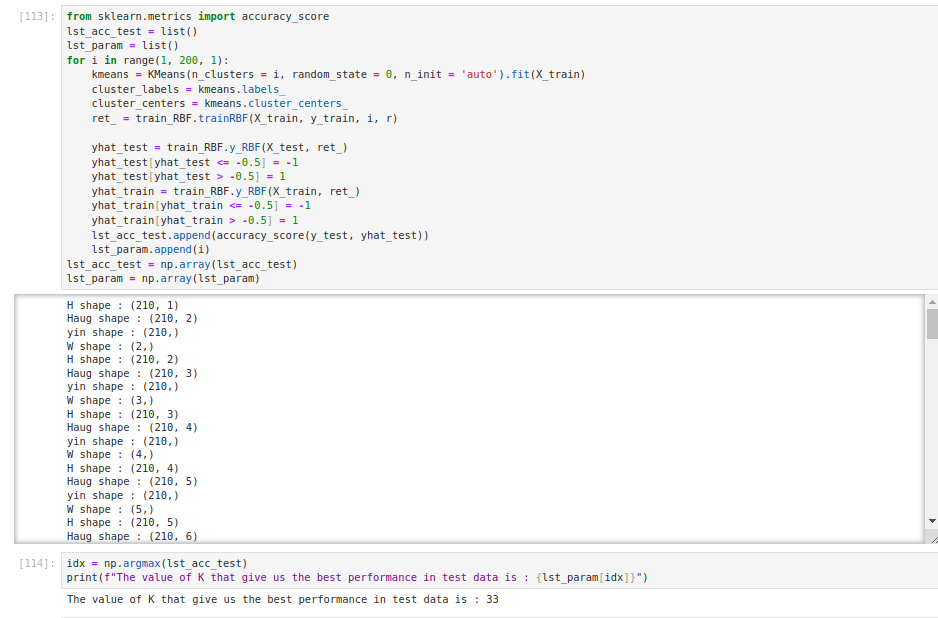
\includegraphics[height=2in]{/home/arthur/Desktop/RNA_BRAGA/ex07/best_k_spirals.png}
                
\end{center}

\vspace{10pt}

\begin{center}

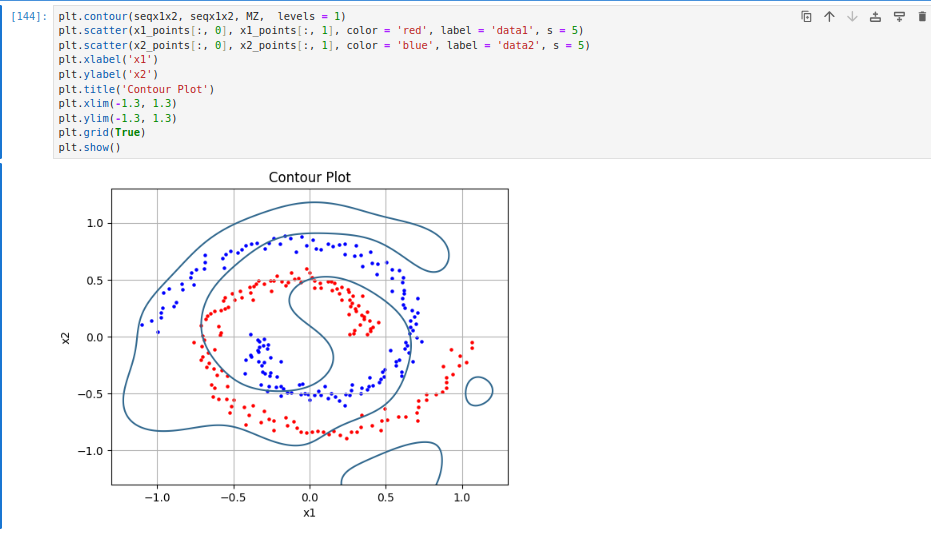
\includegraphics[height=2in]{/home/arthur/Desktop/RNA_BRAGA/ex07/best_k_spirals_plot.png}
                
\end{center}


\vspace{20pt}


\section{Sinc(x)}

\vspace{10pt}

A figura abaixo retrata os dados gerados por uma função sinc(x) com 1 certo ruído gaussiano. Também mostra o resultado do clustering através do algoritmo KMeans :

\vspace{10pt}

\begin{center}

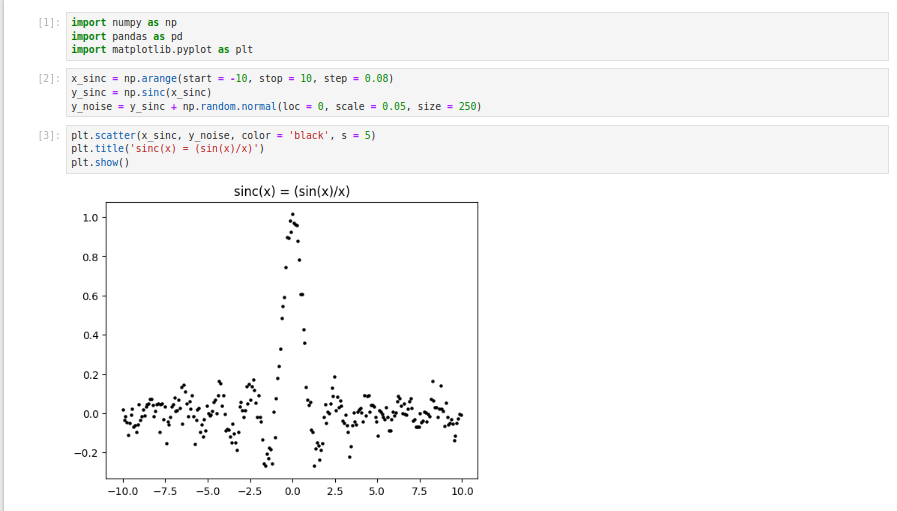
\includegraphics[height=2in]{sinc_data.png}
    
\end{center}

\vspace{10pt}

\begin{center}

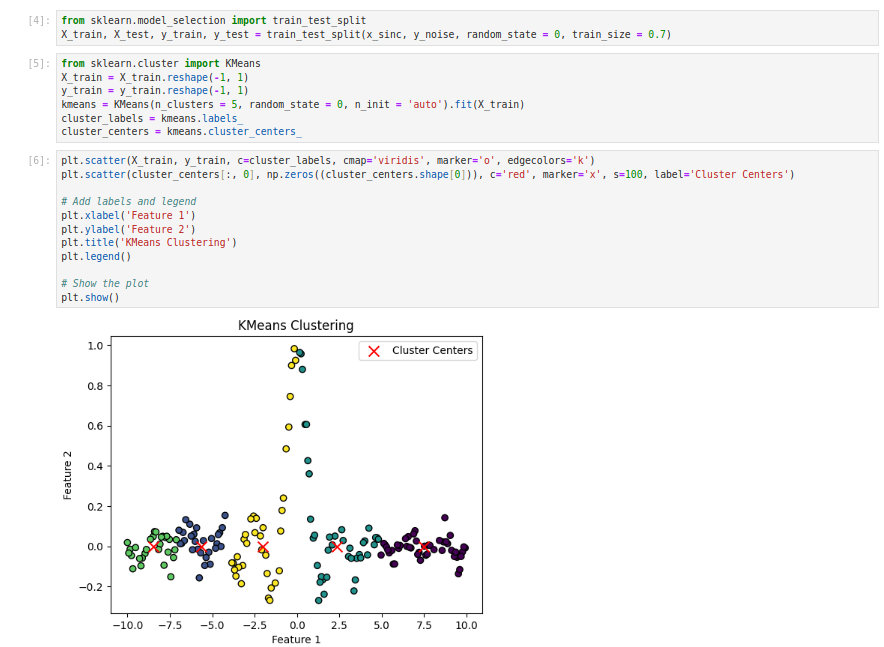
\includegraphics[height=2in]{sinc_cluster.png}
        
\end{center}

\vspace{10pt}

O resultado do erro para K = 5 neurônios está registrado abaixo : 

\vspace{10pt}

\begin{center}

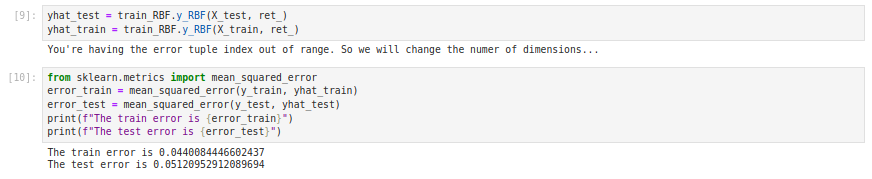
\includegraphics[height=1.5in]{error.png}
    
\end{center}

\vspace{10pt}

O plot abaixo mostra as funções gaussianas utilizadas na camada intermediária, e também a função sinc(x) que gerou os dados.

\vspace{10pt}

\begin{center}

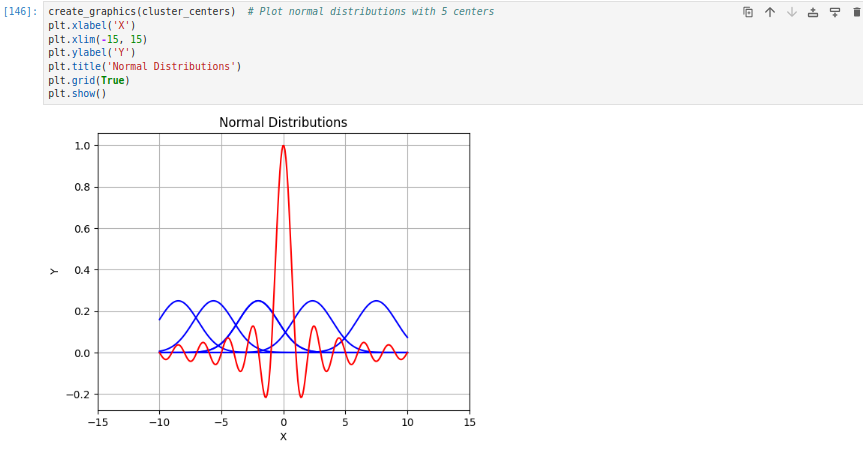
\includegraphics[height=2in]{plot_sinc_gauss.png}
        
\end{center}

\vspace{10pt}

É possível observar que, aumentando o número de funções radiais (neuronios da camada intermediária), o modelo tenderá a ter um overfitting. O valor ideal de K, usando o algoritmo de Grid Search foi de 24 neurônios radiais. A imagem abaixo mostra o algoritmo de Grid Search para encontrar o valor de K o qual o modelo terá a melhor performance.

\vspace{10pt}

\begin{center}

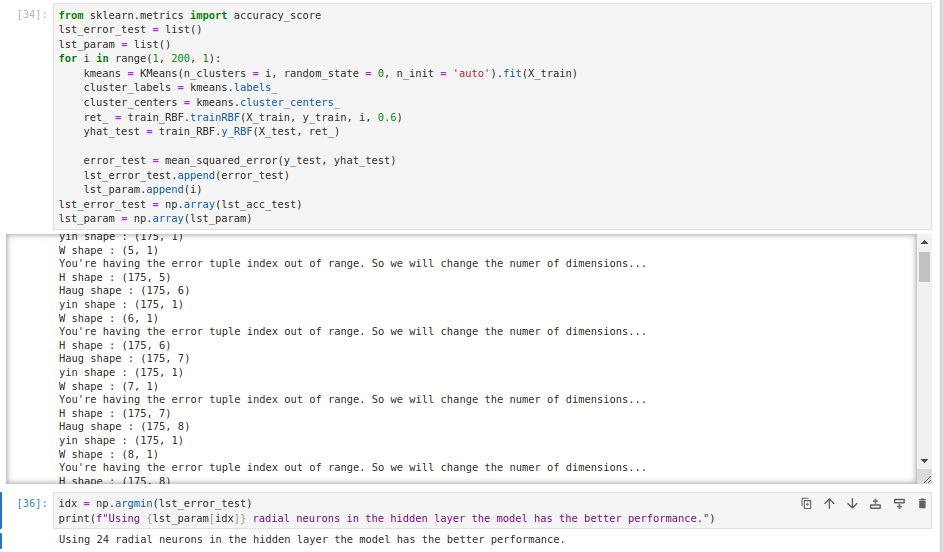
\includegraphics[height=3in]{best_K_sinc.png}
        
\end{center}

\end{document}
